\documentclass[a4paper]{article}
\newtheorem{hyp}{Hypothesis}
\usepackage{graphicx}
\graphicspath{ {/home/angelo/Documents/Uni/Courses/Data Managment & Ethics/Integrated Assignment/assignemnet_project_folder/ERDs/} }


\begin{document}





\title{DME Integrative Assignment}
\author{Angelo Barisano; 508903 }
\date{September 16th, 2022}
\maketitle

\newpage
\section{Task 1: Plan \& Explore: DEfine Questions for project and familiarize with data}

\subsection{Origin of Data \& Purpose Introduction}
\paragraph{Introduction} Data drives security. The wide spread adoption of data information systems has been used to recognize crime-hotspots to increase policing efficiency and protect people. Thus, creating effective information systems for crime prevention is at the center of policy makers and executive branches of governments. This trend has led to the Chicago PD reaching out to this Data Management Team with the request of creating a Data Management System for crime-data in Chicago.

To this end, the Chicago PD and this Data Management Unit is interested on setting the foundation for a FAIR database; i.e. a Data Base ment to flexible and easy in use of slicing and dicing data to find answers and, contemporaneously, make them available. Additiionally, any code produced durign this endeavour will be made public on github for transparency purposes. 

\paragraph{Data description in scope, volumne, and format}
The data was provided by the Chicago PD contains a sample of apprx. 730,000 registered crimes in the administrative districts of Chicago between the years of 2017 and 2021. The initial data source is in csv-format and pertains to specific recroded crimes in the adminsitrative jurisdiction of the Chicago PD in addition to time, location, crime type, and arrested or not. Thus, the data contact is to be found on the Chicago PD website (\textbf{CITE THE CHICAGO WEBSITE FOR THE DATA}). Considerations regarding the ethical (\& GDPR compliant) use of the data will be discussed in part 5 of this assignment.

\paragraph{Project timeframe, researchers, and misc information} The set project timeframe is the 27th of August 2022 till 1st of October 2022. Involved in this project is only one student, Angelo Barisano. Additionally, this project is designed to comply with FAIR standards (\textbf{CITE FAIR STUFF HERE}). Thus, no additional 

\subsection{WHAT IS THE PURPOSE OF THIS ASSIGNMENT??}

\subsection{Research Question}
The overarching goal of this project is to set the foundations to funnel the existing crime-data into a data model to improve its readability (analytics), accessibility (logical structure \& metric-interpretability), and further use in feeding systems for advanced predictive crime prevention. 


\textbf{In an iterative (agile) developmentcylce the following questions have been set up: Chicargo is known for its high homocide rate; this leads to policy makers focusing on this issue the most. }

Upon conducting an initial Exploratory Data Analysis (EDA), three major categories could be identified in the existing data: 

\begin{itemize}
  \item Location
  \item Crime type
  \item Crime record data (time, arrest, etc.)
\end{itemize}

Based on the data types, the EDA, and the aforementioned goal of creating a flexible DB, the following research questions guide the creation of the database in increasing complexity:

\paragraph{Question 1} Finding prevalent crime patterns in the data is a common starting point. Thus, this question provides future research with an adjustable query to gain an overview over the general distribution of crime by type. Subsequently applying a temporal component (i.e. by day of week,  month, year, season, etc.) to this initial distribution reveals trends and temporal patters. This way, this question helps to answer questions to policy makers regarding general trends; such as how crime developed overall and by type. As such, the first question combines the temporal component with the frequency distribution of crime types:

\begin{hyp}[H\ref{hyp:first}] \label{hyp:first}
How do crime types (e.g. homocides) patterns distributed by a temporal component? Are trends observable for different crime types?
How do certain crime types (homicide) patterns distibute by seasonality patterns, by time of day? A specific focus will be laid on policy relevant crimes such as homocides.
\end{hyp}

The aforementioned question(s) enable users to discern trends for crime types in the data. The next logical progression is to add the location dimension to this question. Certain districts and beats tend to be more prevalent in cretain crime types. Thus, question two follows:

\begin{hyp}[H\ref{hyp:second}] \label{hyp:second}
Do certain crime patterns (e.b. for homocides) persist by location such as certain districts/ beats/ blocks?
\end{hyp}

The final step in this analysis is to merge the trend analysis by crime type with the location trends. This analysis by time enables policy makers to discern localized trends in the data in order to address crime patterns by distributing resources more efficiently by alocating resources to necessary districts at certain times of the day. In this context, multiple accessory dimensions will be integrated into the analysis to provide a hollistic description of the situation on the ground. For instance assuming that crimes that lead to more arrests are more frequent in districts/beats by proportion and in total numbers, these crimes put a disproportionate strain on law enforcement. Thus, by triangulating attrests by location, and time of day by season, this will enable us to show areas that need more attention by law enforcement. Another angle would be a specific analysis of beats. Beats are the smallest admininistrative unit of a police district; a beat is patrolled for one year by one unit. Thus, it might be interesting to investigate the connection between a subset of beats that suddenly stop showing problems during one year and then re-appear in terms of crime. The subquestion would, thus, investigate whether beats that usually persisted only persist on a closed yearly basis. This way, effective police units might be identified. This way, the question of resource allocation can be considered. 

As such, the final question considers a variety of hypotheses that can be explored. 

Concluding: 
\begin{hyp}[H\ref{hyp:third}] \label{hyp:third}
Triangualting time, crimetype, and location which areas persit in certain crimes wrt. time?
In order to prevent homocides; which “beats“ are the most prevalent among homcides? During which time of day (for effective allocation of policing resources)? 

\end{hyp}

As such, the final question considers a variety of hypotheses that can be explored. 


Overall, these project based questions are constructed in such a way that they guide an external user (PD) through the process of finding areas that need successively complex "sliced \ diced" information and culminate in the creation of actionable policy implications regarding prime prevention through resource allocation.


\textbf{ADD PLOTS ALREADY HERE!!!}

\section{Design and Organize: Identify and collect the necessary requirements for the databased based on the questions, data and information needs}
In order to address these questions, the relevant information must be broken down into its underlying entities for easier handling. 

\subsection{What entities of importantce to design this database?}
Part 1 identified four borad data categories, which are releveant for this endeavour. At its center, the first information category pertains to the case itself. Connected to cases are the categories of crime type and description in addition to the location category. 
 
 
 
 


Part 1 identified four broad data categories that are of relevance in this endeavour. These categories are the general labels which are defined by different degrees of entities/ complexities. This DB is not only designed for the analysis of the data at hand, but also as a basis for a transactional system to be integrated in a larger framework. Subsequently, "slicing \& dicing" tasks are dependent on the researcher and should not impact future users of the DB.\footnote{This would be an example of setting up tables just for temporary use and then be forgotten or even worse reused for a different purpose: I do not yet know what a future researcher will do. But what I know is how to enable researchers the access to a normed form of data.} As such, the DB is created for general use; Variables are created in views or in scripting languages. 



To start, the location category is defined in decreasing order of complexity by coordinates (lat, lon), beat or sub-district, block, and police district. One district contains multiple beat and blocks.  Thus, this category will be centered by District connected to Block, Beat, and Lat/Lon. \textbf{The reason why Blocks are not placed below Beat hierachically is that there might be some overlap between different Beats patroling the same block. If it turns out that this is not the case, then Blocks will be the hirachically the lowest component below beat.} Finally, Lat/Lon will be connected to District specifically, independent of Beat. This is because this information is technically independent from all other location information. However, the choice to include this category hierachically directly below District was made based for the logical structuring of location data; in a sense: where would you look if you search for Lat/Lon. Additionally, including this relation does not increase the complexity of the querries too much due to the connection of District to the center node Case, which we will discuss next.
\indent The center node of this DB was chosen to be Case. This is because the DB is designed explicitly to only allow recorded crime data, which will improve on the overall data quality; thus, information such as projections or human entered data is minimized as much as possible, so much so that the DB only represents administrative data.\footnote{Synonym for very clean data from a puplic office} The Location category described above is connected to this center node. Every case must have certain location information defined \textbf{(depending on crime; This will be further elaborated upon in part 4 \& 5 when we discuss relation restruictions}. This way, every data entry starts from creating a Case instance, which then can choose the correct Location data. 
\ Beyond Location, every Case requires a crime to be a valid instance. Any crime has a IUCR, which is a code for a combination of a Primary Category of crime, such as murder, and a Secondary Category of a crime, such as first degree murder. Thus, Crime data is connected to Case via IUCR, and IUCR is a code for a primary and secondary relation, defining the crime in question. This way this category is in 3rd NF by design. One might suggest in this context, that IUCR might not be brought up to 3rd NF, as new crimes are rarely added in the penal code and IUCR only contains a total of \textbf{343} instances, while the secondary description entails \textbf{468} and primary description. The rason to bring this category to the 3rd NF is based on 1) the ease of subgroup analysis in one (e.g.) primary category, disregarding any secondary category; i.e. murder is murder after all. Additionally, 2) explicitness and ease of understanding superceeds ease of use in this case. If a new person to the entire Crime sector simply wants to know what penal codes there are, a subanalysis is easier this way. Finally, but not really important, 3) new secondary descriptions would be easier to be added to primary categories.
\indent Furthermore, case specific information will be placed in independent relations, such as Arrests or Location Types. While it might appear that IUCR and Arrest are related, this is technically independent of the Crime description; not every crime leads to a clear cut arrest and is, thus, not mandateted by an IUCR itself. Moreover, Location Type does not describe location specific circumstances pertaining to a Block, Beat, or District but rather the circumstance of how the crime happened. \textbf{This also means, that the name of the Location Type will be changed in the project so to remove any confusion.} 
\indent Finally, any Case requires a Datetime object. This information is placed in the Case instance itself, as the log information is one of the most crucial pieces of information. While some crimes might happen at the same time, normalizing this fact does not make sense with Datetime objects. Views are considerably better suited for "slicing and dicing" the time component than normalizing time, as this project does not have the goal of preimposeing an angle of analysis regarding time.\footnote{it would also be very awkward; I have never seen this case except for panel data. But this is no panel data.} 
\textbf{ARREST SHOULD BE ALSO INCLUDED IN CASE AS A BOOL OR NOT!! }


\subsection{WHAT VARIABLES SHOULD BE INCLUDED???}
\textbf{I DO NOT UNDERSTAND THIS PART? ALL INFORMATION IS SOMEWHAT RELEVANT; MAYBE NO BLOCK INFORMATION; BUT MAYBE IT IS RELEVANT. ADDITIONALLY, for task 3, there are no MANY TO MANY relationships to begin with! So what do they want in aprt 3 from me? WHAT DO YOU MEAN WITH VARIABLES HERE?}




Questions:
1. What do you mean with variables? How can I even design a DB according to the questions in the first place?; eg one question is: do crime pattersn persits over time --> one does not design a database like this; so should I just design the database and then answer the questions with views? in my opinion, one should only build Variables in Views or in Other languages. SQl is a querry language, so this does not make sense to set a variable in the DB. I rather use Views etc. 

\paragraph{Variables} Possible variables created should be used in views. Examples include aggregated crimes by district. Eg average murder per district and then further drilled down to beat; so average murder rate by beat. Then we visualize this fact. Following this we can then see beats that are really fucked up. But I would not create a varaible in the DB. \textbf{In the end we are creating a DB and not a DataWarehouse with prepared variables; Variables should be included in Views and not the database as I do not want to impose a certain variable onto a user of this DB; but views are better suited to this purpose. Databases are meant for raw data and not any transformed data}


\section{Part 3- creation of an entitiy relationship diagram}


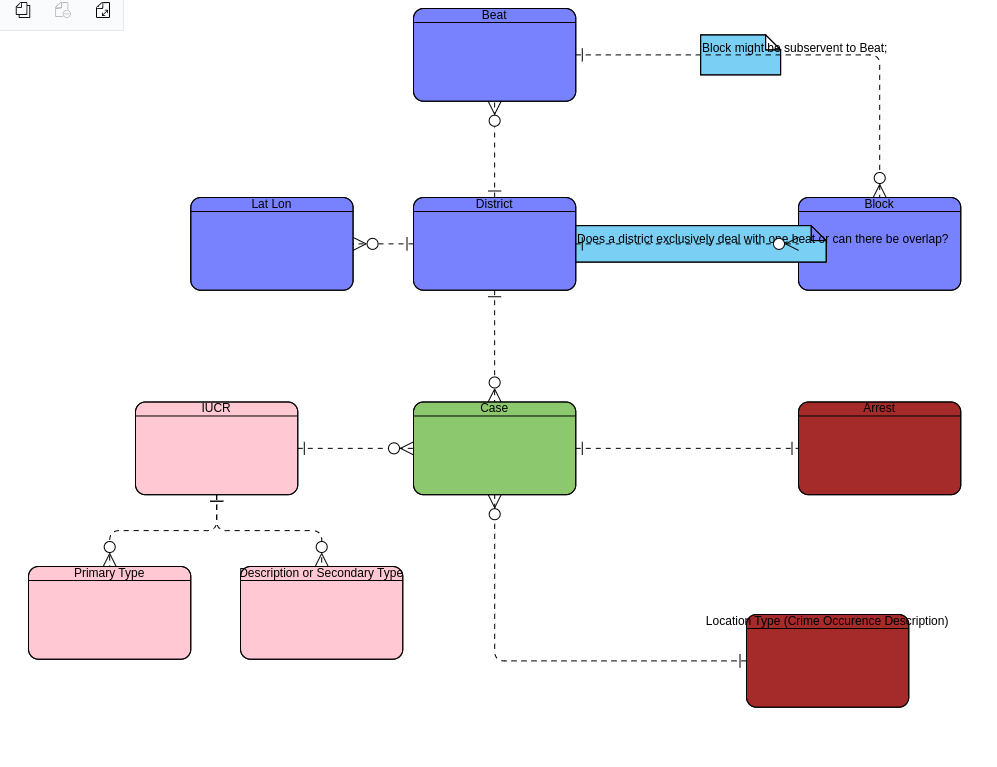
\includegraphics[scale=.35 ]{Conceptual_Model_1.png}


\section{Part 4- Data Quality checks and preparation}
DATA TRIANGLE in lecture!!!



\end{document}
